\documentclass[]{article}
\usepackage[latin1]{inputenc}
\usepackage{amsmath,amssymb,bm} % math stuff


% FOR DISPLAYING CODE
\usepackage{listings}
\usepackage{color}
\definecolor{dkgreen}{rgb}{0,0.6,0}
\definecolor{gray}{rgb}{0.5,0.5,0.5}
\definecolor{mauve}{rgb}{0.58,0,0.82}

\lstset{frame=tb,
	language=Python,
	aboveskip=3mm,
	belowskip=3mm,
	showstringspaces=false,
	columns=flexible,
	basicstyle={\small\ttfamily},
	numbers=none,
	numberstyle=\tiny\color{gray},
	keywordstyle=\color{blue},
	commentstyle=\color{dkgreen},
	stringstyle=\color{mauve},
	breaklines=true,
	breakatwhitespace=true,
	tabsize=4
}

% FOR FIGURES
\usepackage{tikz}
\usetikzlibrary{arrows,calc,positioning,shadows,shapes}


% FOR DISPLAYING HELP BOXES
% Credit goes to Teoman (https://tex.stackexchange.com/questions/66820/how-to-create-highlight-boxes-in-latex)
\usepackage[most]{tcolorbox}
\tcbset{textmarker/.style={%
		enhanced,
		parbox=false,boxrule=0mm,boxsep=0mm,arc=0mm,
		outer arc=0mm,left=6mm,right=3mm,top=7pt,bottom=7pt,
		toptitle=1mm,bottomtitle=1mm,oversize}}
\newtcolorbox{hintBox}{textmarker,
	borderline west={6pt}{0pt}{yellow},
	colback=yellow!10!white}
\newtcolorbox{importantBox}{textmarker,
	borderline west={6pt}{0pt}{red},
	colback=red!10!white}
\newtcolorbox{noteBox}{textmarker,
	borderline west={6pt}{0pt}{green},
	colback=green!10!white}

% define commands for easy access
\newcommand{\note}[1]{\begin{noteBox} \textbf{Note:} #1 \end{noteBox}}
\newcommand{\warning}[1]{\begin{hintBox} \textbf{Warning:} #1 \end{hintBox}}
\newcommand{\important}[1]{\begin{importantBox} \textbf{Important:} #1 \end{importantBox}}




%opening
\title{The guide to Pycle (\textbf{Py}thon \textbf{C}ompresive \textbf{Le}arning toolbox)}
\author{Vincent Schellekens}

\newcommand{\code}{\texttt}
\renewcommand{\Vec}[1]{\bm{#1}} % Pour les vecteurs, re if using amsmath


\begin{document}

% TODO 
% - link to matlab toolbox

\maketitle

\begin{abstract}
	This is the guide to Pycle, a toolbox for Compressive Learning. It is structured as follows: first we shortly explain the theoretical methods this toolbox implements. Then, we explain how the toolbox is structured, and the main steps that a user should follow to use it. The detailed documentation of all the functionalities in the toolbox is then provided, followed by some practical examples to get started easily.
\end{abstract}


\section{What is Compressive Learning?}
% TODO


		
\begin{figure}[!htb]
	\centering
	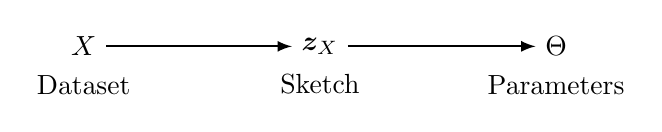
\begin{tikzpicture}
	% Place nodes
	\node [label=below:Dataset] (dataset) at (0,0) {$X$};
	\node [label=below:Sketch] (sketch) at (3,0) {$\Vec{z}_X$};
	\node [label=below:Parameters] (parameters) at (6,0) {$\Theta$};
	
	% Draw edges
	\draw [->, thick, -latex] (dataset) -- (sketch);
	\draw [->, thick, -latex] (sketch) -- (parameters);
	\end{tikzpicture}
	\caption{Compressive learning .}
	\label{fig:CL}
	\end {figure}


\begin{equation}
\label{eq:sketching}
	\Vec{z}_X := \frac{1}{n} \sum_{i = 1}^n \Phi(\Vec{x}_i)
\end{equation}

See \cite{gribonval2017compressive} for a complete introduction to compressive learning.

\section{An overview of Pycle}
% TODO explain how it is structured, how to use


\subsection{Requirements}
The Pycle package builds on a set of standard Python libraries, that are required to run it: % standard in scientific computing with python
\begin{itemize}
	\item \code{numpy}
	\item \code{scipy}
	\item \code{matplotlib}
\end{itemize}

% You can install those packages by...

\subsection{Typical workflow}

A typical use of Pycle follows the following steps:
\begin{enumerate}
	\item Design a sketch operator, then sketch the dataset using the \code{sketching.py} module.
	\item Extract a model from the sketch by a compressive learning method contained in the \code{compressive\_learning.py} module.
\end{enumerate}




	
		
\begin{figure}[!htb]
	\centering
		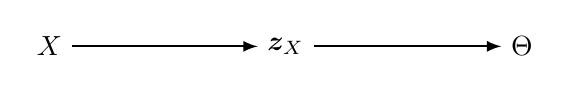
\begin{tikzpicture}
		% Place nodes
		\node (dataset) at (0,0) {$X$};
		\node (sketch) at (3,0) {$\Vec{z}_X$};
		\node (parameters) at (6,0) {$\Theta$};
		
		% Draw edges
		\draw [->, thick, -latex] (dataset) -- (sketch);
		\draw [->, thick, -latex] (sketch) -- (parameters);
		\end{tikzpicture}
	\caption{Flowchart of a typical compressive learning execution with Pycle.}
	\label{fig:flowchart}
\end {figure}
		



\section{A tutorial tour of \code{pycle}}

\subsection{Sketching} 
To use the \code{sketching} submodule, you first need to import it (I personally like \code{sk} as shorthand). Usual sketching as defined in~\eqref{eq:sketching} can then be done by calling \code{sk.computeSketch} as follows.
\begin{lstlisting}
import pycle.sketching as sk

X = ...    # load a numpy array of dimension (n,d)
Phi = ... # sketch feature map, see later

z = sk.computeSketch(X,Phi)
\end{lstlisting}

As you might have guessed, \code{sk.computeSketch(dataset,featureMap)} requires two arguments, the dataset encoded as a numpy array, and the feature map $\Phi$.

\note{\textbf{Dataset representation conventions}.
In \code{pycle}, we follow the mainstream convention for datasets, where a collection of $a$ vectors in dimension $b$ is encoded as a numpy array of size $(a,b)$. Thus, the dataset $X = (\Vec{x}_i \in \mathbb R^d)_{i = 1}^n$ is a $(n,d)$ numpy array (even when $d = 1$) which means that \code{X[0]} references $\Vec{x_1}$. Similarly, the projection matrix $\Omega = (\Vec{\omega}_j \in \mathbb R^d)_{j = 1}^m$ is a $(m,d)$ array, etc.}

The feature map argument can be specified in one of the two following ways. Either you give an instance of a \code{FeatureMap} object, which we explain below, or you directly provide a custom callable function (e.g., to compute the second-order moments for the sketch, write \code{Phi = lambda x: x**2}).

\note{\textbf{FeatureMap objects}. TO CHANGE
At this point, you might be wondering why we bother to construct a \code{FeatureMap} object instead of a function to represent... well, a (mathematical) function, namely $\Phi$. The reason is that actual learning algorithms (from \code{pycle.compressive\_learning}) or even other sketching functionalities (e.g., privacy preservation) require not just the ability to evaluate $\Phi$ but other information about it (e.g., its target dimension $m$, its jacobian $\nabla\Phi$, whether it belongs to a set of standard maps etc.). Those informations are packaged in the \code{FeatureMap} object for your convenience.}



% Motivation

\subsection{Learning} 

\subsection{Utilities} 


\section{Documentation}
\subsection{Sketching methods} 

\subsection{Learning tools} 

\subsection{Utilities} 

\section{Examples}
% TODO some examples, or put notebooks instead?


\newpage
\bibliography{guidebib.bib}
\bibliographystyle{ieeetr}


\end{document}
